\documentclass[10pt]{article}
\usepackage{icmlko}

\icmlmeta{IP 파운데이션 월드모델}{7}{굽은 길과 곧은 길}{문서에서 축으로는 비선형, 축에서 결과로는 선형 --- 레인 하나가 노트 5와 6을 갈랐다}

\begin{document}

\twocolumn[
\icmlheader

\begin{abstract}
노트 6은 열린 충돌 하나를 남겼다. 다섯 축 태그를 트리 모델에 넣은 팔이 반복 분할에서
상수에 졌는데(승률 10\%), 노트 5는 같은 프로토콜에서 같은 다섯 축이 40회 중 40회
이겼다고 보고했다. 재현해 보니 \textbf{원인은 레인 하나였다} --- 같은 축, 같은 75건,
같은 분할에서 ridge는 승률 100\%(차이 $-$0.0354), 트리는 15\%(차이 $+$0.0276)다.
둘 다 옳았고 모델류가 달랐을 뿐이다. 여기서 세 가지가 따라 나온다. 첫째,
\textbf{다섯 축의 신호는 선형이다} --- 제곱과 상호작용 항을 얹을수록 성능이 단조로
무너지며, 15차원 상호작용에서 승률 33\%로 붕괴한다. 둘째, \textbf{노트 5의 ``축을
데이터로 발견할 수 없다''는 결론은 레인 탓이었다} --- ridge로 폴드 안에서 고르게 하면
선택률 상위 여섯 중 다섯이 노트 4가 지목한 다섯이고, 트리에서 전 폴드 선택되던 콜라보
강도는 0.375로 일곱 번째로 밀린다. 셋째, 그럼에도 \textbf{구조는 비대칭이어야 한다} ---
신경망 헤드를 선형으로 바꾸면 좋아지지만(차이 $+$0.0275$\to$$+$0.0056) 인코더까지
선형으로 벗기면 오히려 무너진다($+$0.0571, 승률 0\%). 문서에서 축으로 가는 길은
굽어 있고, 축에서 결과로 나오는 길은 곧다.
\end{abstract}
]

\section{충돌에서 시작한다}

노트 6은 앵커된 다섯 슬롯 구조를 짓고, 마지막에 정직하게 미결로 남긴 항목이 있었다.

\begin{quote}\fontsize{9.2}{11}\selectfont
열린 충돌: 다섯 축 태그를 트리 모델에 그대로 넣은 팔이 반복 분할에서 상수에 졌다
(중앙 $+$0.036, 승률 10\%). 노트 5는 같은 프로토콜에서 고정 5종이 40회 중 40회
이겼다고 보고했다.
\end{quote}

두 수치는 같은 75건, 같은 IP 무작위 5폴드, 같은 타깃에서 나왔다. 그런데 부호가
반대다. 둘 중 하나는 틀렸거나, 아니면 내가 같다고 여긴 무언가가 실은 달랐다.

노트 5의 반복 CV는 인라인으로 실행돼 코드가 남지 않았다. 그래서 재현부터 했다.
차이가 날 수 있는 축을 전부 열었다 --- 피처 표현(원값 대 0--1 정규화), 마스크 컬럼
유무, 표본 가중치 유무, 그리고 레인.

\section{레인 하나가 부호를 뒤집는다}

첫 네 조합에서 답이 나왔다.

\begin{table}[t]
\centering\tsize
\caption{같은 다섯 축, 같은 75건, IP 무작위 5폴드 40회 반복.}
\begin{tabular}{llrrr}
\toprule
피처 집합 & 레인 & 차이 중앙 & 표준편차 & 이긴 비율 \\
\midrule
고정 5종 & ridge & $-$0.0354 & 0.011 & \textbf{100\%} \\
고정 5종 & 트리  & $+$0.0276 & 0.025 & 15\% \\
기획 10종 & ridge & $-$0.0079 & 0.015 & 70\% \\
기획 10종 & 트리  & $+$0.0063 & 0.023 & 42\% \\
\bottomrule
\end{tabular}
\end{table}

\begin{figure}[t]
\centering
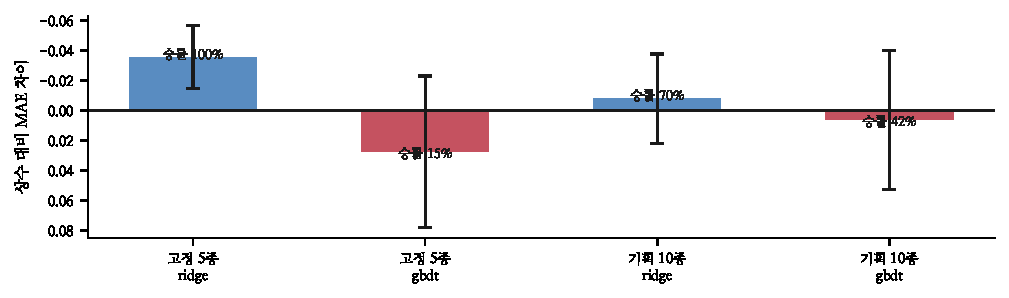
\includegraphics[width=\textwidth]{figs/lane_gap.pdf}
\caption{레인을 바꾸면 결론이 뒤집힌다. 노트 5는 왼쪽 첫 막대를, 노트 6의 2단 실험은
두 번째 막대를 보고 있었다. 오차 막대는 반복 표준편차의 두 배다.}
\end{figure}

노트 5는 ridge를, 노트 6의 2단 실험은 트리를 썼다. 둘 다 맞았다. 충돌은 사라졌지만
훨씬 중요한 질문이 남았다 --- \emph{왜 선형 모델만 이 신호를 보는가.}

\claimx{같은 다섯 축이 선형 모델에서는 40회 중 40회 상수를 이기고 트리 모델에서는
40회 중 6회만 이긴다. 레인은 구현 세부가 아니라 결론을 정하는 선택이다.}{표본을
두 배로 늘렸을 때 트리가 ridge를 따라잡으면 원인은 신호의 형태가 아니라 표본
크기였던 것이다.}

\section{신호는 선형이다}

가설 둘을 가른다. 신호가 실제로 선형이어서 트리가 헛돈 것인가, 아니면 신호는
비선형인데 n=75에서 트리가 그것을 학습하지 못한 것인가.

다섯 축에 제곱 항과 상호작용 항을 단계적으로 얹고 같은 ridge로 재본다. 신호에
비선형 성분이 있다면 확장이 도움이 돼야 한다.

\begin{table}[t]
\centering\tsize
\caption{다섯 축의 비선형 확장. ridge, IP 무작위 5폴드 40회 반복.}
\begin{tabular}{lrrr}
\toprule
확장 & 차원 & 차이 중앙 & 이긴 비율 \\
\midrule
\textbf{선형만} & 5 & \textbf{$-$0.0354} & \textbf{100\%} \\
$+$제곱 & 10 & $-$0.0267 & 95\% \\
$+$상호작용 & 15 & $+$0.0071 & 33\% \\
전부 & 20 & $-$0.0061 & 57\% \\
\bottomrule
\end{tabular}
\end{table}

\begin{figure}[t]
\centering
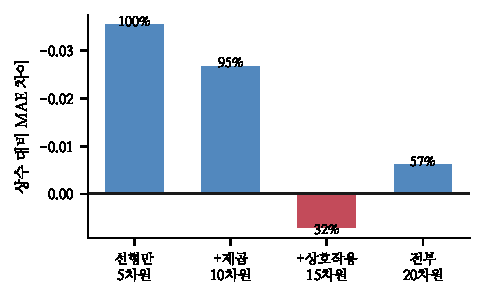
\includegraphics[width=\columnwidth]{figs/linearity.pdf}
\caption{비선형 항을 더할수록 무너진다. 막대 위 숫자는 40회 중 상수를 이긴 비율이다.
상호작용 열 항이 가장 해롭다.}
\end{figure}

확장은 도움이 되지 않았고 상호작용은 결정적으로 해로웠다. 다만 이 결과가
``비선형 성분이 없다''를 증명하지는 못한다 --- 학습 폴드가 60건인데 상호작용만
열 개를 더하면 어떤 신호든 묻힌다. 정확히 말할 수 있는 것은 \emph{현재 표본에서
비선형 항은 이득이 없고, 선형 항만 남기는 것이 최선}이라는 사실이다.

\claimx{현재 표본에서 다섯 축은 선형으로 쓰는 것이 최선이며, 제곱과 상호작용을
더하면 단조로 나빠진다.}{표본이 커진 뒤 상호작용 항이 순수 선형을 이기면, 신호는
원래 비선형이었고 n=75가 감당하지 못한 것이다.}

\section{노트 5의 ``발견 불가''를 다시 본다}

노트 5의 핵심 주장은 이랬다 --- 폴드마다 다른 다섯을 고르므로 축을 데이터로부터
발견할 수 없다. 그 근거로 든 것이 콜라보 강도였다. 네 폴드 전부에서 선택됐는데
노트 4는 그것을 제거 대상으로 지목했으므로, 같은 데이터가 정반대 답을 낸다는
증거로 삼았다.

그 중첩 선택의 레인이 기록되지 않았다. ridge로 다시 돌렸다. IP 무작위 5폴드
8회 반복, 학습 폴드 안에서만 leave-one-out으로 열 개를 다섯으로 줄인다.

\begin{figure}[t]
\centering
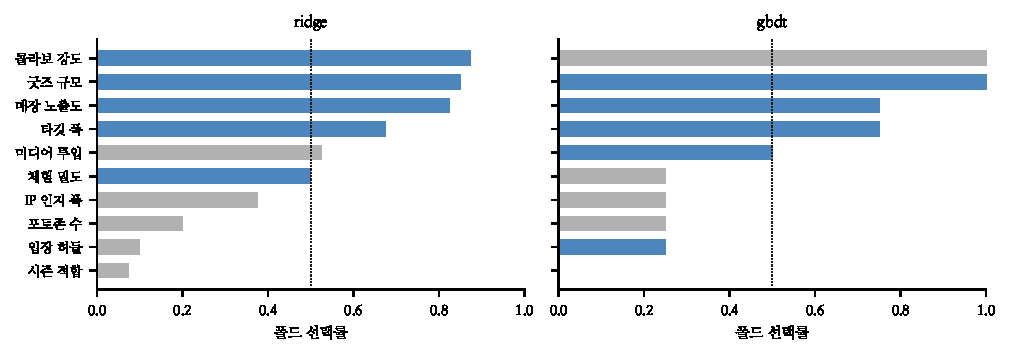
\includegraphics[width=\textwidth]{figs/select_lane.pdf}
\caption{폴드 선택률. 진한 막대가 노트 4가 지목한 다섯이다. ridge에서는 상위 여섯 중
다섯이 그 다섯이고, 트리에서 공동 1위였던 콜라보 강도는 0.375로 밀린다.
점선은 절반이다.}
\end{figure}

\begin{table}[t]
\centering\tsize
\caption{ridge 폴드 선택률 (40 폴드). 굵은 것이 노트 4의 다섯.}
\begin{tabular}{lr@{\hspace{2em}}lr}
\toprule
속성 & 선택률 & 속성 & 선택률 \\
\midrule
\textbf{타깃 폭}     & \textbf{0.875} & 콜라보 강도  & 0.375 \\
\textbf{굿즈 규모}   & \textbf{0.850} & 시즌 적합    & 0.200 \\
\textbf{매장 노출도} & \textbf{0.825} & IP 인지 폭   & 0.100 \\
\textbf{입장 허들}   & \textbf{0.675} & 체험 밀도    & 0.075 \\
포토존 수            & 0.525 & & \\
\textbf{미디어 투입} & \textbf{0.500} & & \\
\bottomrule
\end{tabular}
\end{table}

ridge에서 데이터는 노트 4의 다섯을 거의 정확히 가리킨다. 유일한 침입자는 포토존
수(0.525)가 미디어 투입(0.500)을 간발로 앞선 것뿐이다. 노트 5가 모순의 증거로 든
콜라보 강도는 0.375로 일곱 번째다.

\paragraph{그러나 절반만 철회한다}
축의 \emph{정체}는 ridge에서 회복된다. 그런데 폴드마다 새로 고르는 \emph{절차}는
여전히 상수를 이기지 못한다(차이 $+$0.0019, 승률 50\%). 고정해 쓰면 100\%
이기는데도 그렇다. 선택 절차 자체가 분산원이기 때문이다.

그래서 노트 5의 두 문장은 이렇게 갈라진다.

\begin{quote}\fontsize{9.2}{11}\selectfont
\textbf{철회.} ``데이터가 그 다섯을 알려줄 수 없다'' --- 알려줄 수 있다. 선형
레인에서 선택률이 명확히 그 다섯을 가리킨다.\\[0.35em]
\textbf{유지.} ``폴드마다 새로 고르면 이득이 사라진다'' --- 그대로다. 선택은
한 번만 하고 고정해야 한다.
\end{quote}

\claimx{축을 데이터로 식별하는 것과 매 폴드에서 다시 고르는 것은 다르다. 앞은
선형 레인에서 가능하고, 뒤는 어느 레인에서도 손해다. 한 번 고르고 고정하라.}{독립
표본에서 ridge 선택률 상위 다섯이 이 다섯과 어긋나면 식별 가능성 주장은 무너진다.}

\section{구조는 비대칭이어야 한다}

노트 6의 신경망은 상수를 이기지 못했다(승률 25\%). 신호가 선형이라면 원인은 명백해
보였다 --- 헤드가 MLP, 즉 비선형이었다. 비선형을 한 겹씩 벗기며 재봤다.

\begin{table}[t]
\centering\tsize
\caption{선형 사다리. 앵커 16, IP 무작위 5폴드 20회 반복.}
\begin{tabular}{lrrr}
\toprule
구조 & 차이 중앙 & 표준편차 & 이긴 비율 \\
\midrule
MLP 인코더 $+$ MLP 헤드   & $+$0.0275 & 0.025 & 25\% \\
\textbf{MLP 인코더 $+$ 선형 헤드} & \textbf{$+$0.0056} & 0.020 & \textbf{35\%} \\
선형 인코더 $+$ 선형 헤드  & $+$0.0571 & 0.026 & 0\% \\
선형(항등) $+$ 선형 헤드   & $+$0.1638 & 0.057 & 0\% \\
\bottomrule
\end{tabular}
\end{table}

\begin{figure}[t]
\centering
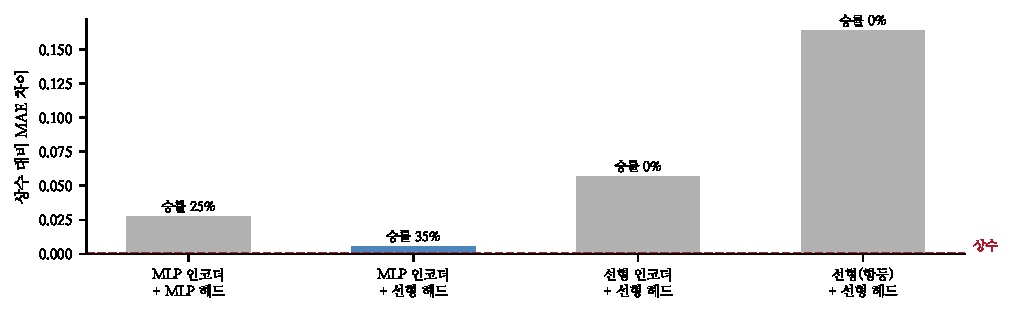
\includegraphics[width=\textwidth]{figs/ladder.pdf}
\caption{비선형을 벗기는 순서가 중요하다. 헤드를 벗기면 좋아지고 인코더까지 벗기면
무너진다. 예측이 반증된 지점이다.}
\end{figure}

앞쪽 절반은 예측대로였다. 헤드를 선형으로 바꾸자 결손이 절반 아래로 줄었다
($+$0.0275 $\to$ $+$0.0056). 그런데 인코더까지 선형으로 벗기자 오히려 크게
나빠졌다($+$0.0571, 20회 중 0회 승리). 시그모이드마저 뗀 항등 사상은 $+$0.1638로
완전히 무너졌다.

\emph{내 예측은 절반만 맞았다.} ``신호가 선형이니 전부 선형으로''는 틀렸다. 맞는
문장은 이것이다.

\begin{itemize}[leftmargin=1.1em,itemsep=0.15em]
\item \textbf{문서 $\to$ 축}은 비선형이다. ``타깃 폭''이나 ``입장 허들'' 같은
      의미 축은 문서의 수치들로부터 임계와 범주를 거쳐 만들어진다. 선형 사상으로는
      복원되지 않는다.
\item \textbf{축 $\to$ 결과}는 선형이다. 축이 주어지면 결과는 그 합으로 설명된다.
\end{itemize}

\claimx{앵커된 슬롯 구조에서 인코더는 비선형이어야 하고 헤드는 선형이어야 한다.
둘을 같은 종류로 맞추면 어느 쪽으로 맞추든 나빠진다.}{인코더를 선형으로 두고도
비선형 인코더와 같은 성능이 나오면, 문서에서 축으로 가는 길이 굽었다는 진단이
틀린 것이다.}

\section{그래서 다음 질문}

이 비대칭은 새 질문을 만든다. 인코더가 실제로 문서에서 축을 얼마나 복원하는가.
ridge가 100\%로 이기는 이유가 선형이어서가 아니라 \emph{사람이 매긴 축을 그대로
받기 때문}이라면, 앵커 구조의 병목은 헤드가 아니라 인코더다. 그리고 그것이 사실이면
함의가 크다 --- 사람 태깅은 문서의 중복 정보가 아니라 새 정보이고, 아이돌 도메인
전이는 아이돌 태깅 없이는 불가능하며, 파운데이션 모델의 입력은 문서가 아니라 태그여야
한다.

폴드 밖에서 문서만으로 각 축을 예측해 사람 태그와 대조하는 측정을 돌리고 있다.
다음 노트의 주제다.

\section{한계}

\begin{itemize}[leftmargin=1.1em,itemsep=0.15em]
\item 비선형 확장 실험은 ``비선형 성분이 없다''를 증명하지 못한다. 학습 폴드 60건에
      상호작용 열 개는 어떤 신호든 묻는다. 표본이 커진 뒤 재측정해야 한다.
\item ridge 선택률은 8회 반복 40 폴드에서 나왔다. 트리 쪽 비교는 노트 5의 시간순
      4폴드 결과를 그대로 썼으므로 폴드 수가 다르다. 트리 쪽 반복 재계산은 중첩
      leave-one-out 비용 때문에 아직 돌고 있다.
\item 기획 10종의 반복 CV 수치가 노트 5(차이 $-$0.0290, 98\%)와 이번 재현
      ($-$0.0079, 70\%)에서 어긋난다. 마스크 컬럼과 정규화를 포함한 32개 변형
      전수 비교를 돌리고 있으며, 결과에 따라 노트 5의 해당 수치를 정정한다.
      고정 5종 수치는 노트 5($-$0.0442, 100\%)와 재현($-$0.0354, 100\%)이
      부합하므로 이 노트의 결론에는 영향이 없다.
\item 모든 반복 분할은 시간 순서를 쓰지 않는다. 실전 성능이 아니라 안정성 판정용이다.
\end{itemize}

\section{다음}

\begin{enumerate}[leftmargin=1.3em,itemsep=0.15em]
\item 축 복원 검정 --- 문서만으로 다섯 축을 얼마나 맞히는가. 앵커 구조의 병목 확정.
\item 32개 변형 전수 비교 완료 후 노트 5 수치 정정.
\item 태그 순열 대조군 --- 노트 6이 남긴 반증 조건.
\item 아이돌 다섯 축 태깅. 축 복원이 어렵다는 결과가 나오면 이것은 선택이 아니라 필수다.
\end{enumerate}

\vspace{0.6em}
\hrule height 0.3pt
\vspace{0.5em}
{\footnotesize
\textbf{참고문헌}\\[0.3em]
Grinsztajn, L., Oyallon, E., Varoquaux, G. (2022). Why do tree-based models still
outperform deep learning on typical tabular data? \emph{NeurIPS 2022}.\\[0.15em]
Hastie, T., Tibshirani, R., Friedman, J. (2009). \emph{The Elements of Statistical
Learning}, 2nd ed. Springer.\\[0.15em]
Hollmann, N. et al. (2025). Accurate predictions on small data with a tabular
foundation model. \emph{Nature}, 637, 319--326.\\[0.15em]
Varma, S., Simon, R. (2006). Bias in error estimation when using cross-validation
for model selection. \emph{BMC Bioinformatics}, 7, 91.
}

\end{document}
